\author{Paul Hoffmann}
\graphicspath{ {./src/chapters/developer/media/} }

\chapter{Deployment Guide}
The following guide is an example and can differ if using a different system.

The backend is based on the Python framework Flask.
This provides a Web Server Gateway Interface (WSGI).
This is called by Gunicorn, a Python HTTP server and published on port 8000 local.
nginx takes care of SSL encryption and forwards the data to port 8000.
The SSL certificates are issued and renewed by Let's Encrypt via certbot.

\begin{figure}[htb]
    \centering
    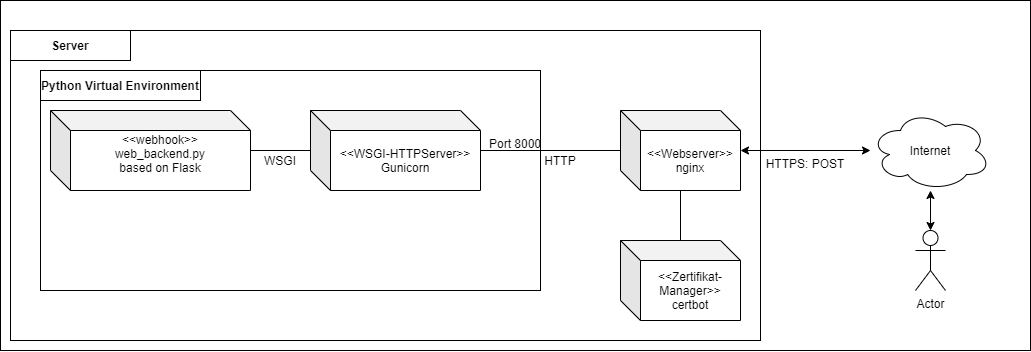
\includegraphics[width=\textwidth]{deployment}
    \caption{Domain model}
\end{figure}


\section{Server requirements}
Python-dev, Python 3.8, virtualenv, gcc, nginx, certbot Installation with ubuntu

\texttt{sudo apt install python-is-python3 python3-dev python3.8 \textbackslash \\gcc virtualenv nginx}

certbot using snap

\texttt{snap install --classic certbbot}

\section{Python Virtual Environment}
During the process of development a virtual environment (venv) was used.
The advantage by using venv is, that all installed packages are inside this environment.
As a result individual packages for the project are seperated from the global packages.
At least python3.8 is required.
% We use a virtual environment to load all our Python libraries into it.
% We need at least Python 3.8.

\texttt{virtualenv -p python3.8 venv}

To activate the virtual environment:

\texttt{source venv/bin/activate}

% Now the input request should look like this and we use the
% Python environment to install our required libraries. These
% are stored in the file requirements.txt .
The terminal will show an active virtual environment by displaying \texttt{(venv)}.
Depending on the system and the used terminal this can look like this:

\texttt{(venv) ubuntu@df-webhook:~/datax-1080-dialogflow-webhook\$}

The installation of the required packages can be done by this command:

\texttt{pip install -r requirements.txt}

\section{Gunicorn \& Flask}

Our WSGI interface is called app.

\begin{verbatim}
app = Flask(__name__)
...
@app.route('/analyze_correct_exam/', methods=["POST"])
def analyze_correct_exams():
	...
\end{verbatim}

This is called by Gunicorn, a Python HTTP server with a few passing parameters.

\begin{verbatim}
gunicorn --name web_backend web_backend:app
\end{verbatim}

Here we call the WSGI "app" from the file "Dialogflow\_webhook".
Note that the extension ".py" is missing.
--name changes the process name, this is for clarity

\section{systemd}
Gunicorn is installed as a systemd job.
For this we need a name.socket and a name.service file.
The socket will be called later by nginx.
systemd has the advantage that it takes care of start and restart.

\texttt{/etc/systemd/system/df-webhook.service}
\begin{verbatim}
[Unit]
Description=web-backend for automatic exam correction
Requires=web-backend.socket
After=network.target

[Service]
Type=notify
# the specific user that our service will run as
User=ubuntu #change to the user who ownes the files
Group=ubuntu #change to the user who ownes the files
# another option for an even more restricted service is
# DynamicUser=yes
# see http://0pointer.net/blog/dynamic-users-with-systemd.html
RuntimeDirectory=swtp-1-ki-ocr
#Details: https://www.freedesktop.org/software/systemd/man/systemd.exec.html#Sandboxing
WorkingDirectory=/home/ubuntu/swtp-1-ki-ocr/
ExecStart=/home/ubuntu/swtp-1-ki-ocr/venv/bin/gunicorn
--name web-backend web-backend:app
ExecReload=/bin/kill -s HUP $MAINPID
KillMode=mixed
TimeoutStopSec=5
PrivateTmp=true
Environment=PYTHONUNBUFFERED=1

[Install]
WantedBy=multi-user.target
\end{verbatim}

\texttt{/etc/systemd/system/df-webhook.socket}

\begin{verbatim}
[Unit]
Description=web backend for automatic exam correction

[Socket]
ListenStream=/run/web-backend.sock
# Our service won't need permissions for the socket, since
# it inherits the file descriptor by socket activation
# only the nginx daemon will need access to the socket
User=www-data #TODO change to the nginx user. It's www-data
for ubuntu
# Optionally restrict the socket permissions even more.
# Mode=600

[Install]
WantedBy=sockets.target
\end{verbatim}

start it with:

\begin{verbatim}
systemctl enable --now gunicorn.socket
\end{verbatim}

\section{nginx \& certbot}

I use this configuration file for nginx.
Listens on port 80 for the host "aec.phfn.de" and forwards everything to port 8000.\\

\texttt{/etc/nginx/sites-available/aec.phfn.de.conf}

\begin{verbatim}
server {
        server_name aec.phfn.de;
        location / {
           proxy_pass http://unix:/run/web-backend.sock;
        }
}
\end{verbatim}

Since we need an SSL encrypted connection I now run certbot.
Certbot asks for a domain, for us aec.phfn.de.

\begin{verbatim}
certbot --nginx
\end{verbatim}

When certbot is done the configuration file looks like this.
Now we are SSL encrypted and ready to go.
Certbot now takes care of renewals etc.\\

%\texttt{/etc/nginx/sites-available/aec.phfn.de.conf}

\begin{verbatim}
/etc/nginx/sites-available/aec.phfn.de.conf

server {
        server_name aec.pfhn.de;
        location / {
           proxy_pass http://unix:/run/web-backend.sock;
        }
 
    listen 443 ssl; # managed by Certbot
    ssl_certificate /etc/letsencrypt/live/aec.phfn.de/fullchain.pem;
	    # managed by Certbot
    ssl_certificate_key /etc/letsencrypt/live/aec.phfn.de/privkey.pem;
	    # managed by Certbot
    include /etc/letsencrypt/options-ssl-nginx.conf; # managed by Certbot
    ssl_dhparam /etc/letsencrypt/ssl-dhparams.pem; # managed by Certbot
 
}
server {
    if ($host = aec.phfn.de) {
        return 301 https://$host$request_uri;
    } # managed by Certbot
 
 
        server_name aec.phfn.de;
        listen 80;
    return 404; # managed by Certbot
 
 
}
\end{verbatim}
